\chapter{अम्ल, क्षारक और pH}\label{ch:g9:acids-bases-ph}

रसोई की एक शेल्फ़ पर एक नींबू, सिरके की एक बोतल, साबुन की एक टिकिया और
खाने के सोडे का एक डिब्बा रखा है; सिंक के नीचे काले और लाल चेतावनी लेबल
वाली नाली-साफ़ करने वाले घोल की एक बोतल है। इनमें से कुछ का स्वाद खट्टा है,
कुछ छूने में फिसलन भरे लगते हैं, कुछ त्वचा को जला सकते हैं। 0 से 14 तक
अंकित एक ही पैमाना इन सबको छाँट देता है --- और यही पैमाना तरणतालों, बगीचे की
मिट्टी, रक्त और महासागरों के लिए भी इस्तेमाल होता है।

\begin{recall}
\omterm{def:g9:ions:ion}{आयन} ऐसे \omterm{def:g7:atoms-and-molecules:atom}{परमाणु} या \omterm{def:g7:atoms-and-molecules:atom}{परमाणुओं} के समूह हैं जिन पर आवेश होता है; \ce{Na+} जैसा
\omterm{def:g9:ions:ion}{धनायन} धनात्मक होता है, \ce{Cl-} या \ce{OH-} जैसा \omterm{def:g9:ions:ion}{ऋणायन} ऋणात्मक।
आयनिक विलयनों में (aq) से चिह्नित \omterm{def:g9:ions:ion}{आयन} होते हैं, जो स्वतंत्र रूप से घूमते हैं
(\cref{ch:g9:ions})।
\end{recall}

\begin{omfigure}
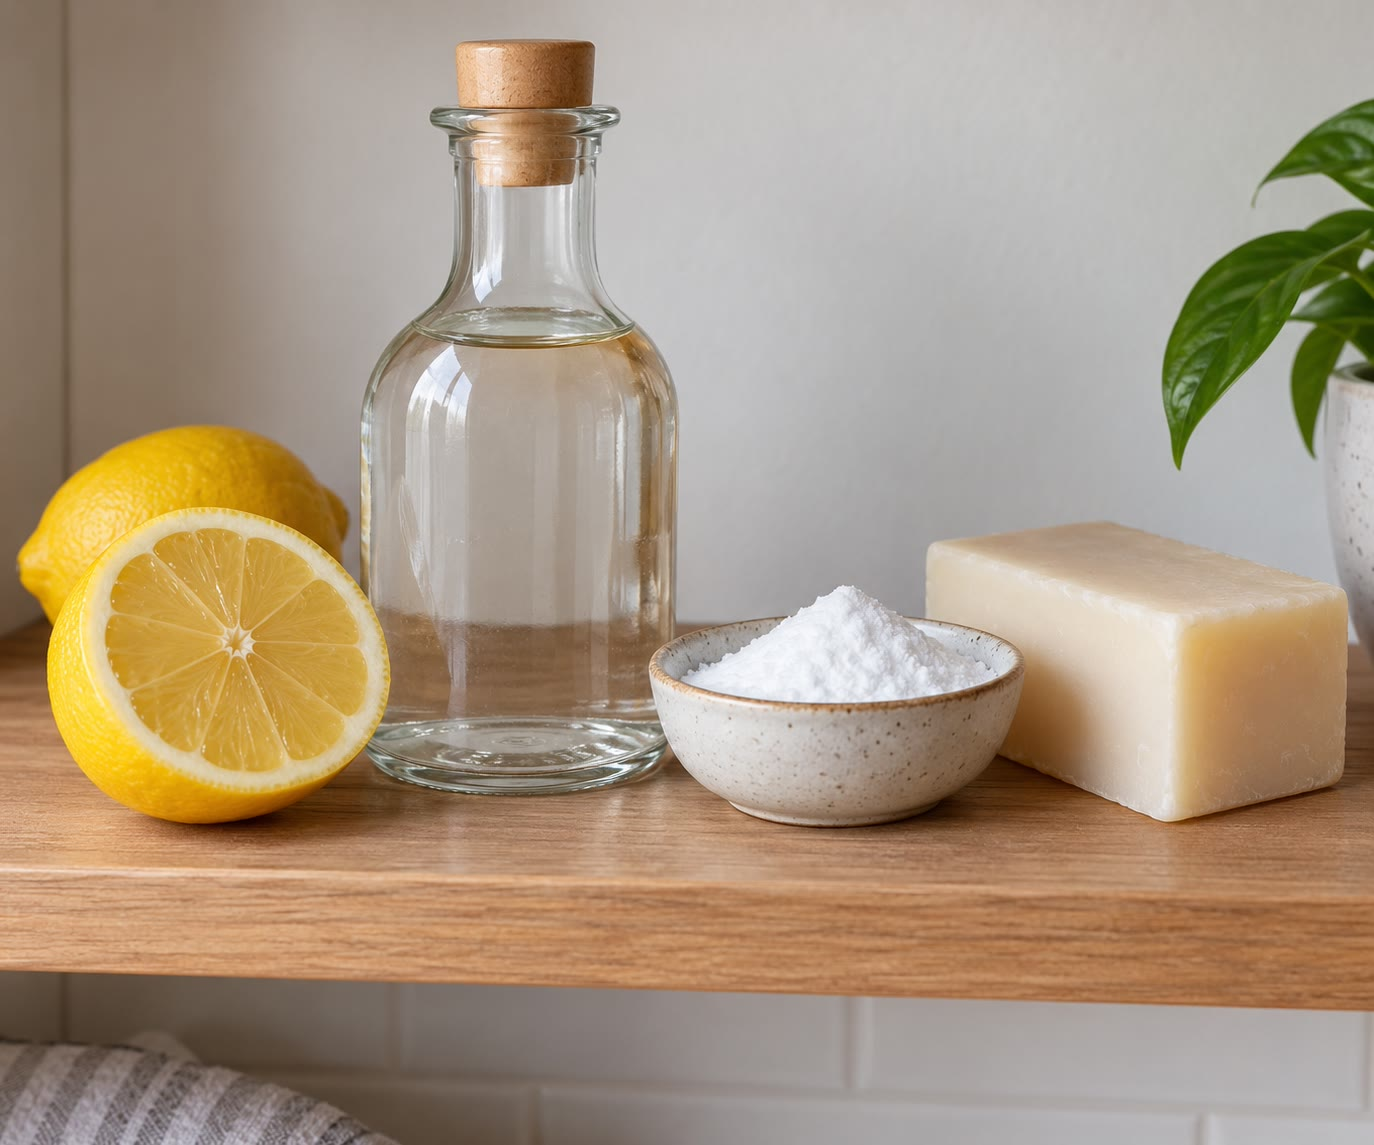
\includegraphics[width=0.55\linewidth]{images/book1/ai/g9-kitchen-shelf.jpg}

{\small नींबू, सिरका, साबुन और खाने का सोडा: रसोई में अम्ल और
क्षारक।}
\end{omfigure}

\section{अम्लीय, क्षारकीय और उदासीन विलयन}

\begin{definition}[अम्लीय, क्षारकीय और उदासीन विलयन]\label{def:g9:acids-bases-ph:acidic}
हर \omterm{def:g6:solutions-and-solubility:solute}{जलीय विलयन} में हाइड्रोजन \omterm{def:g9:ions:ion}{आयन} \ce{H+(aq)} और हाइड्रॉक्साइड
\omterm{def:g9:ions:ion}{आयन} \ce{OH-(aq)} होते हैं। कोई विलयन \emph{अम्लीय विलयन}\index{अम्लीय विलयन}
होता है जब उसमें \ce{H+} \omterm{def:g9:ions:ion}{आयन} \ce{OH-} \omterm{def:g9:ions:ion}{आयनों} से अधिक हों,
\emph{क्षारकीय विलयन}\index{क्षारकीय विलयन} होता है जब उसमें
\ce{OH-} \omterm{def:g9:ions:ion}{आयन} \ce{H+} \omterm{def:g9:ions:ion}{आयनों} से अधिक हों, और \emph{उदासीन
विलयन}\index{उदासीन विलयन} होता है जब दोनों बराबर संख्या में हों।
\end{definition}

\begin{example}[तीन विलयन]\label{ex:g9:acids-bases-ph:three}
हाइड्रोक्लोरिक अम्ल एक \omterm{def:g9:acids-bases-ph:acidic}{अम्लीय विलयन} है: उसमें \ce{H+(aq)} और
\ce{Cl-(aq)} \omterm{def:g9:ions:ion}{आयन} होते हैं, \ce{OH-} बहुत कम। सोडियम हाइड्रॉक्साइड का विलयन
क्षारकीय है: \ce{Na+(aq)} और \ce{OH-(aq)}, \ce{H+} बहुत कम। शुद्ध
पानी और नमकीन पानी उदासीन हैं।
\end{example}

\section{pH पैमाना}

\begin{definition}[pH]\label{def:g9:acids-bases-ph:ph}
किसी \omterm{def:g6:solutions-and-solubility:solute}{जलीय विलयन} का \emph{pH}\index{pH} एक संख्या है, आम तौर पर
0 और 14 के बीच, जो बताती है कि वह कितना अम्लीय या क्षारकीय है:
\qty{25}{\celsius} पर \omterm{def:g9:acids-bases-ph:acidic}{उदासीन विलयन} का pH 7 होता है, \omterm{def:g9:acids-bases-ph:acidic}{अम्लीय विलयन} का pH
7 से कम, \omterm{def:g9:acids-bases-ph:acidic}{क्षारकीय विलयन} का pH 7 से अधिक। विलयन में जितने अधिक \ce{H+} \omterm{def:g9:ions:ion}{आयन}
होते हैं, उसका pH उतना ही कम होता है।
\end{definition}

\begin{omfigure}
\begin{tikzpicture}[font=\small, x=0.95cm]
  \foreach \k in {0,...,13} {
    \pgfmathtruncatemacro\rr{2.2*max(0,100-14.3*\k)+30}
    \pgfmathtruncatemacro\gg{1.8*(\k<7 ? 30+10*\k : 100-8*(\k-7))+40}
    \pgfmathtruncatemacro\bb{2.2*max(0,14.3*(\k-6))+30}
    \definecolor{phc}{RGB}{\rr,\gg,\bb}
    \fill[phc] (\k,0) rectangle ++(1,0.6);
  }
  \foreach \k in {0,...,14} \node[anchor=north, font=\footnotesize] at (\k,-0.02) {\k};
  \draw[black!60] (0,0) rectangle (14,0.6);
  \node[anchor=south] at (3.5,0.65) {अम्लीय};
  \node[anchor=south] at (7,0.65) {उदासीन};
  \node[anchor=south] at (10.5,0.65) {क्षारकीय};
  % ledger: ph:HCl-1M, ph:gastric, ph:lime, ph:wine, ph:coffee, ph:pure-water, ph:seawater, ph:milk-magnesia, ph:ammonia, ph:NaOH-1M
  \foreach \x/\lab/\lev/\anc in {0/{हाइड्रोक्लोरिक\\ अम्ल (1 M)}/1/north, 1.5/{जठर\\ रस}/3/north east,
      2/{कागज़ी नींबू\\ का रस}/2/north west, 3.5/{वाइन}/1/north, 5/{कॉफ़ी}/2/north, 7/{शुद्ध\\ पानी}/3/north,
      8.1/{समुद्र का\\ पानी}/1/north, 10.5/{मिल्क ऑफ़\\ मैग्नीशिया}/3/north, 12/{घरेलू\\ अमोनिया}/1/north,
      14/{सोडियम हाइड्रॉक्साइड\\ (1 M)}/2/north east} {
    \draw[black!55] (\x,-0.45) -- (\x,-0.45-0.8*\lev);
    \node[anchor=\anc, font=\footnotesize, align=center, inner sep=2pt] at (\x,-0.45-0.8*\lev) {\lab};
  }
\end{tikzpicture}

{\small \omterm{def:g9:acids-bases-ph:ph}{pH} पैमाना, कुछ आम विलयनों के \omterm{def:g9:acids-bases-ph:ph}{pH} के साथ।}
\end{omfigure}

\begin{definition}[pH पत्र और pH मीटर]\label{def:g9:acids-bases-ph:ph-paper}
\emph{pH पत्र}\index{pH पत्र} कागज़ की एक पट्टी है, जिसे रंजकों के एक
\omterm{def:g6:pure-substances-and-mixtures:mixture}{मिश्रण} में भिगोया गया है और जो हर \omterm{def:g9:acids-bases-ph:ph}{pH} पर अलग रंग लेती है; विलयन की एक बूँद
उस पर रखी जाती है और रंग की तुलना डिब्बे पर छपे चार्ट से की जाती है।
\emph{pH मीटर}\index{pH मीटर} विलयन में डुबोए गए काँच के एक प्रोब से \omterm{def:g9:acids-bases-ph:ph}{pH}
मापता है और उसे एक या दो दशमलव स्थानों तक एक संख्या के रूप में
दिखाता है।
\end{definition}

\begin{method}[pH पत्र से pH मापना]\label{met:g9:acids-bases-ph:paper}
\begin{enumerate}
  \item \omterm{def:g9:acids-bases-ph:ph-paper}{pH पत्र} की एक छोटी पट्टी एक साफ़, सूखी तश्तरी पर रखो।
  \item एक साफ़ काँच की छड़ से पट्टी पर विलयन की एक बूँद छुआओ (पट्टी को
        कभी बोतल में मत डुबोओ)।
  \item तुरंत रंग की तुलना चार्ट से करो, और \omterm{def:g9:acids-bases-ph:ph}{pH} पढ़ो,
        आम तौर पर निकटतम पूर्ण संख्या तक।
\end{enumerate}
\end{method}

\begin{omfigure}
\begin{tikzpicture}[font=\small, scale=1.2]
  \pic[transform shape] at (0,0) {stirrer};
  \pic[transform shape] at (0,0.05) {beaker={0.55}{omWater!80}};
  \pic[transform shape] at (0.25,0.35) {probe};
  \pic[transform shape] at (2.6,3.4) {meter={pH}};
  \draw[black!70, line width=0.6pt] (0.25,3.45) .. controls (0.3,4.3) and (2.2,4.4)
    .. (2.2,2.95);
  \draw[<-, omProp, thick] (0.4,1.0) -- (2.0,1.3) node[right, text=black] {काँच का प्रोब};
  \draw[<-, omProp, thick] (3.35,3.4) -- (4.0,3.4) node[right, text=black] {pH मीटर};
  \draw[<-, omProp, thick] (-0.6,0.6) -- (-1.6,0.9) node[left, text=black] {विलयन};
\end{tikzpicture}

{\small \omterm{def:g9:acids-bases-ph:ph-paper}{pH मीटर} से \omterm{def:g9:acids-bases-ph:ph}{pH} मापना: काँच का प्रोब विलयन में डूबा है, जिसे धीरे-धीरे
चलाया जा रहा है।}
\end{omfigure}

\section{अम्ल को तनु करना}

\begin{proposition}[तनु करने से pH 7 के क़रीब आता है]\label{prop:g9:acids-bases-ph:dilution}
\omterm{def:g9:acids-bases-ph:acidic}{अम्लीय विलयन} में पानी मिलाने से उसके \ce{H+} \omterm{def:g9:ions:ion}{आयन} बड़े आयतन में फैल जाते हैं:
\omterm{def:g9:acids-bases-ph:ph}{pH} बढ़ता है, 7 की ओर, पर उससे आगे कभी नहीं। हाइड्रोक्लोरिक अम्ल जैसे
अम्ल के लिए दस गुना तनु करने से \omterm{def:g9:acids-bases-ph:ph}{pH} लगभग एक इकाई बढ़ता है: \omterm{def:g9:acids-bases-ph:ph}{pH} 2 वाले अम्ल
का एक आयतन और पानी के नौ आयतन मिलकर \omterm{def:g9:acids-bases-ph:ph}{pH} 3 का विलयन देते हैं। इसी तरह
\omterm{def:g9:acids-bases-ph:acidic}{क्षारकीय विलयन} को तनु करने से उसका \omterm{def:g9:acids-bases-ph:ph}{pH} घटकर 7 की ओर
आता है।
\end{proposition}

\begin{omfigure}
\begin{tikzpicture}[font=\small, scale=1.05]
  \foreach \k/\ph/\cc in {0/2/red!38!omWater,1/3/red!24!omWater,2/4/red!12!omWater} {
    \pic[transform shape] at (\k*4.4,0) {beaker={0.55}{\cc}};
    \node[anchor=north, align=center] at (\k*4.4,-0.15) {pH \ph};
  }
  \foreach \k in {0,1} \draw[->, thick, omProp] (\k*4.4+1.1,1.0) -- (\k*4.4+3.3,1.0)
    node[midway, above, text=black, font=\footnotesize, align=center]
    {10 mL + 90 mL\\ पानी};
\end{tikzpicture}

{\small अम्ल को दस गुना तनु करना, फिर दोबारा दस गुना: \omterm{def:g9:acids-bases-ph:ph}{pH} 2 से 3 और फिर 4
हो जाता है (हर बीकर पिछले विलयन का दसवाँ भाग है, जिसमें पानी मिलाकर
आयतन पूरा किया गया है)।}
\end{omfigure}

\begin{inthelab}[अम्ल को तनु करना]
अम्ल को तनु करने के लिए शिक्षक हमेशा अम्ल को धीरे-धीरे पानी में डालते हैं,
पानी को अम्ल में कभी नहीं: मिलाने पर ऊष्मा निकलती है, और सांद्र अम्ल पर डाला
गया पानी तुरंत उबलकर अम्ल को बर्तन से बाहर
उछाल सकता है।
\end{inthelab}

\section{रोज़मर्रा के अम्ल और क्षारक}

\begin{proposition}[हमारे आस-पास के अम्ल और क्षारक]\label{prop:g9:acids-bases-ph:everyday}
अम्लीय: नींबू और कागज़ी नींबू का रस, सिरका, वाइन, सोडा वाले पेय, कॉफ़ी,
पेट का जठर रस। क्षारकीय: समुद्र का पानी (थोड़ा-सा), पानी में घुला खाने का
सोडा, साबुन, मिल्क ऑफ़ मैग्नीशिया (पेट की अम्लता की एक दवा), घरेलू अमोनिया,
ब्लीच, नाली साफ़ करने वाला घोल (बहुत तेज़)।
\end{proposition}

\begin{example}[महासागर का pH]\label{ex:g9:acids-bases-ph:ocean}
% ledger: ph:seawater, ph:ocean-drop
महासागर का औसत \omterm{def:g9:acids-bases-ph:ph}{pH} लगभग 8.1 है: थोड़ा क्षारकीय। औद्योगिक युग शुरू होने के
बाद से \omterm{def:g4:air-a-mixture-of-gases:air}{वायु} से \omterm{def:g2:mixing-and-dissolving:dissolve}{घुलती} कार्बन डाइऑक्साइड ने सतही जल का \omterm{def:g9:acids-bases-ph:ph}{pH} लगभग 0.1 घटा दिया
है: महासागर धीरे-धीरे कम क्षारकीय होते जा रहे हैं, जिससे सीपों वाले जीवों
और प्रवालों को हानि पहुँचती है।
\end{example}

\begin{omfigure}
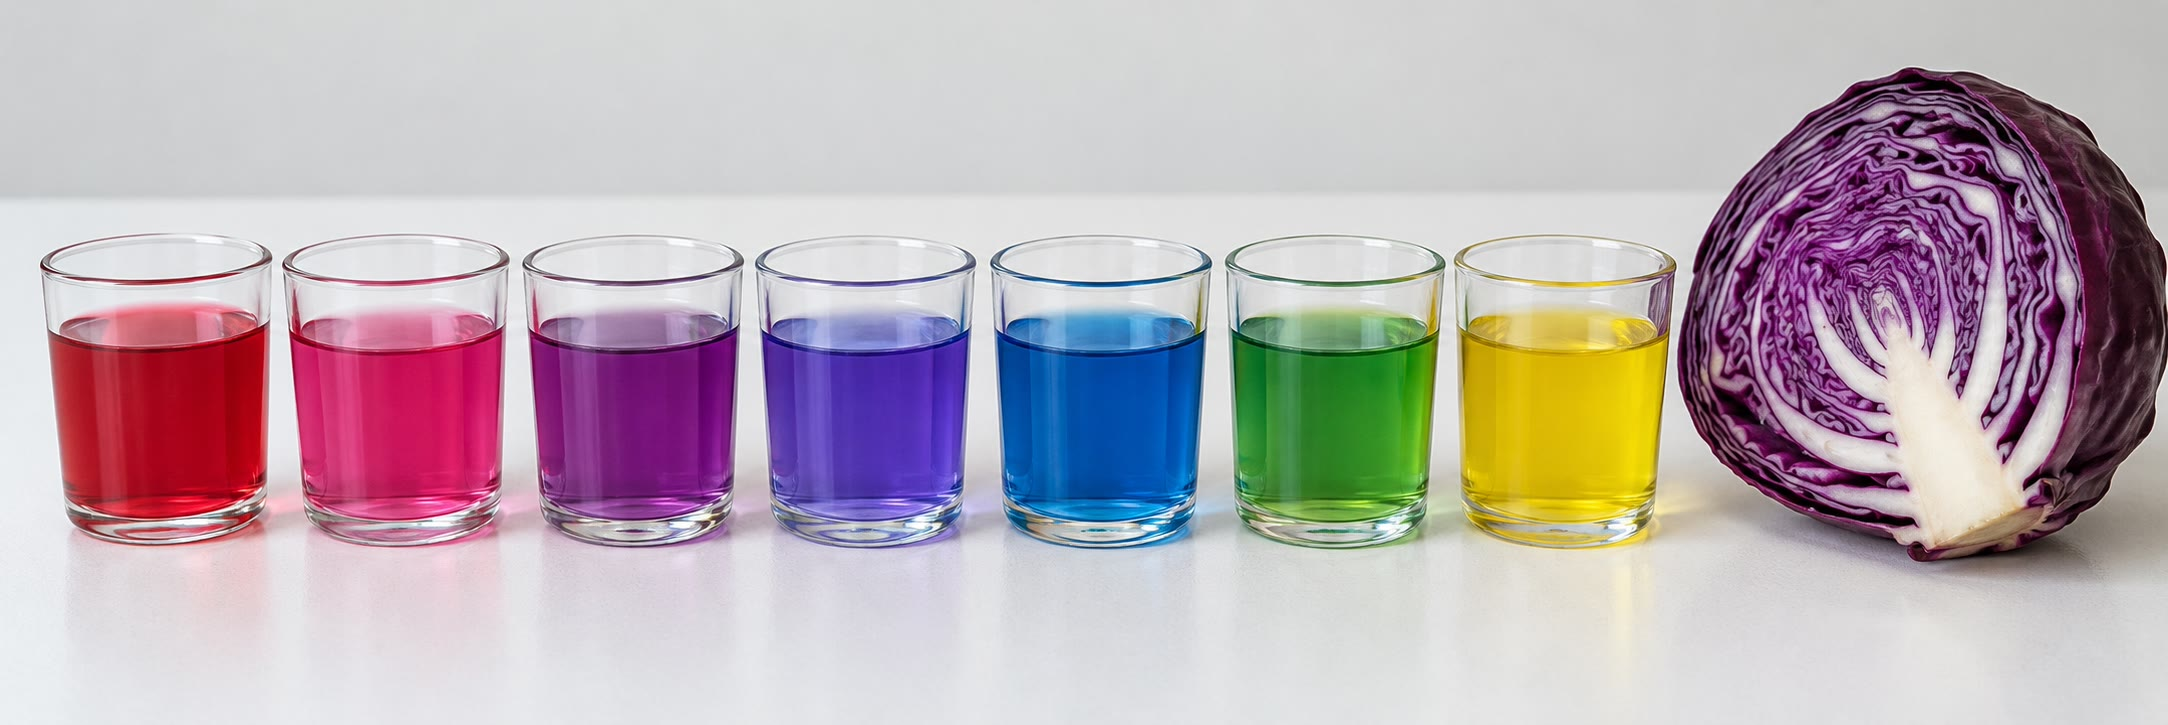
\includegraphics[width=0.55\linewidth]{images/book1/ai/g9-red-cabbage.jpg}

{\small शिक्षक द्वारा तैयार किया गया लाल पत्तागोभी का रस \omterm{def:g9:acids-bases-ph:ph}{pH} के साथ रंग बदलता है:
अम्लों में लाल, उदासीन के पास बैंगनी, और अधिकाधिक \omterm{def:g9:acids-bases-ph:acidic}{क्षारकीय विलयनों} में
नीला, हरा, फिर पीला।}
\end{omfigure}

\section{संक्षारक उत्पादों के साथ सुरक्षा}

\begin{safety}{\ghs[0.85cm]{GHS05}\ghs[0.85cm]{GHS07}}
% ledger: ghs:HCl, ghs:NaOH
सांद्र हाइड्रोक्लोरिक अम्ल और सोडियम हाइड्रॉक्साइड (नाली साफ़ करने वाले घोलों का
क्षारक) पर संक्षारण चित्रसंकेत GHS05 होता है: वे त्वचा और आँखों को गंभीर रूप से
जलाते हैं और धातुओं पर आक्रमण करते हैं। GHS07: उत्तेजक। चश्मा और दस्ताने;
छींटा पड़ने पर तुरंत ढेर सारे पानी से धोया जाता है।
\end{safety}

\begin{remark}[सफ़ाई के उत्पादों को कभी न मिलाएँ]\label{rem:g9:acids-bases-ph:mix}
अम्लीय और क्षारकीय उत्पाद आपस में अभिक्रिया करते हैं, कभी-कभी तीव्रता से, और कुछ
\omterm{def:g6:pure-substances-and-mixtures:mixture}{मिश्रणों} से विषैली गैसें निकलती हैं: ब्लीच को अम्लीय डीस्केलर के साथ मिलाने पर
क्लोरीन निकलती है। सफ़ाई के उत्पाद कभी नहीं मिलाए जाते।
\end{remark}

\section{अभ्यास}

\begin{exercise}[$\star$]\label{exo:g9:acids-bases-ph:1}
अम्लीय, क्षारकीय या उदासीन? \omterm{def:g9:acids-bases-ph:ph}{pH} 3 वाला विलयन, \omterm{def:g9:acids-bases-ph:ph}{pH} 7 वाला, \omterm{def:g9:acids-bases-ph:ph}{pH} 11
वाला।
\end{exercise}

\begin{exercise}[$\star$]\label{exo:g9:acids-bases-ph:2}
\omterm{def:g9:acids-bases-ph:acidic}{अम्लीय विलयन} में कौन-से \omterm{def:g9:ions:ion}{आयन} अधिक होते हैं? क्षारकीय में?
\end{exercise}

\begin{exercise}[$\star$]\label{exo:g9:acids-bases-ph:3}
इस अध्याय के \omterm{def:g9:acids-bases-ph:ph}{pH} पैमाने की मदद से सबसे अम्लीय से सबसे क्षारकीय के क्रम में
लगाओ: कॉफ़ी, समुद्र का पानी, कागज़ी नींबू का रस, घरेलू अमोनिया, शुद्ध
पानी।
\end{exercise}

\begin{exercise}[$\star$]\label{exo:g9:acids-bases-ph:4}
\omterm{def:g9:acids-bases-ph:ph-paper}{pH पत्र} से किसी विलयन का \omterm{def:g9:acids-bases-ph:ph}{pH} मापने का तरीका बताओ।
\end{exercise}

\begin{exercise}[$\star\star$]\label{exo:g9:acids-bases-ph:5}
\omterm{def:g9:acids-bases-ph:ph}{pH} 4 वाले विलयन को पानी से दस गुना तनु किया जाता है। उसका नया \omterm{def:g9:acids-bases-ph:ph}{pH} लगभग कितना
है? और अगर उसे सौ गुना तनु किया जाए तो?
\end{exercise}

\begin{exercise}[$\star\star$]\label{exo:g9:acids-bases-ph:6}
क्या पानी मिलाकर कोई \omterm{def:g9:acids-bases-ph:acidic}{अम्लीय विलयन} क्षारकीय बन सकता है? समझाओ।
\end{exercise}

\begin{exercise}[$\star\star$]\label{exo:g9:acids-bases-ph:7}
अम्ल को पानी में ही क्यों डालना चाहिए, उलटा क्यों नहीं?
\end{exercise}

\begin{exercise}[$\star\star$]\label{exo:g9:acids-bases-ph:8}
एक बोतल पर GHS05 चित्रसंकेत है। इसका क्या अर्थ है? दो
सावधानियाँ बताओ।
\end{exercise}

\begin{exercise}[$\star\star$]\label{exo:g9:acids-bases-ph:9}
किसी अम्ल को \omterm{def:g9:acids-bases-ph:ph}{pH} 1 से \omterm{def:g9:acids-bases-ph:ph}{pH} 4 तक ले जाने के लिए कितने दस-गुना तनुकरण चाहिए?
यह कुल कितना तनुकरण है?
\end{exercise}

\begin{exercise}[$\star\star$]\label{exo:g9:acids-bases-ph:10}
पेट की अम्लता के लिए मिल्क ऑफ़ मैग्नीशिया लिया जाता है। \omterm{def:g9:acids-bases-ph:ph}{pH} पैमाने की मदद से
समझाओ क्यों।
\end{exercise}

\begin{exercise}[$\star\star\star$]\label{exo:g9:acids-bases-ph:11}
औद्योगिक युग से अब तक महासागर का \omterm{def:g9:acids-bases-ph:ph}{pH} लगभग 0.1 घटा है। क्या आज महासागर
अम्लीय है? वह किस दिशा में बढ़ रहा है, और क्यों?
\end{exercise}

\begin{exercise}[$\star\star\star$]\label{exo:g9:acids-bases-ph:12}
एक छात्र उसी सिरके का \omterm{def:g9:acids-bases-ph:ph}{pH} \omterm{def:g9:acids-bases-ph:ph-paper}{pH पत्र} से (3) और \omterm{def:g9:acids-bases-ph:ph-paper}{pH मीटर} से (2.6) मापता है।
समझाओ कि दोनों परिणाम अलग क्यों हैं और कौन-सा अधिक
परिशुद्ध है।
\end{exercise}

\section{समस्या: अम्ल का गिरना}

\begin{problem}[{सप्ताहांत समस्या --- प्रयोगशाला के सिंक में गिरा एक लीटर अम्ल,
और उसे तनु करना हल क्यों नहीं है}]
\label{pb:g9:acids-bases-ph:1}
\omterm{def:g9:acids-bases-ph:ph}{pH} 2 वाले तनु हाइड्रोक्लोरिक अम्ल की \qty{1}{L} से भरी एक बोतल प्रयोगशाला के
सिंक में टूट जाती है। नाली में \omterm{def:g9:acids-bases-ph:ph}{pH} 5 से कम वाला कोई भी विलयन नहीं जाना
चाहिए। इस अध्याय का नियम लो: इस अम्ल के लिए हर दस-गुना
तनुकरण \omterm{def:g9:acids-bases-ph:ph}{pH} को एक इकाई बढ़ाता है।

\medskip
\noindent\textbf{भाग I --- अम्ल।}
\begin{enumerate}
  \item विलयन अम्लीय है, उदासीन या क्षारकीय? उसमें कौन-से \omterm{def:g9:ions:ion}{आयन} सबसे
        अधिक हैं?
  \item बोतल पर कौन-सा चित्रसंकेत होना चाहिए, और क्यों?
  \item शिक्षक \omterm{def:g9:acids-bases-ph:ph-paper}{pH पत्र} के बजाय \omterm{def:g9:acids-bases-ph:ph-paper}{pH मीटर} से \omterm{def:g9:acids-bases-ph:ph}{pH} मापते हैं।
        एक लाभ बताओ।
  \item उसी अम्ल के \omterm{def:g9:acids-bases-ph:ph}{pH} 2 वाले एक लीटर में \omterm{def:g9:acids-bases-ph:ph}{pH} 3 वाले एक लीटर की तुलना में
        कितने गुना \ce{H+} \omterm{def:g9:ions:ion}{आयन} हैं?
\end{enumerate}

\medskip
\noindent\textbf{भाग II --- तनु करना।}
\begin{enumerate}[resume]
  \item एक लीटर अम्ल को दस गुना तनु करने पर विलयन का कितना आयतन मिलता है?
        उसका \omterm{def:g9:acids-bases-ph:ph}{pH} क्या है?
  \item \omterm{def:g9:acids-bases-ph:ph}{pH} 5 तक पहुँचने के लिए कितने दस-गुना तनुकरण चाहिए?
  \item तब विलयन का कुल आयतन कितना होगा?
  \item क्या पानी की कोई भी मात्रा विलयन को क्षारकीय बना सकती है? समझाओ।
\end{enumerate}

\medskip
\noindent\textbf{भाग III --- एक बेहतर तरीका।}
इसके बजाय शिक्षक किसी क्षारक का विलयन थोड़ा-थोड़ा तब तक मिलाते हैं जब तक
\omterm{def:g9:acids-bases-ph:ph-paper}{pH पत्र} 7 न दिखाए: अम्ल के \ce{H+} \omterm{def:g9:ions:ion}{आयन} क्षारक के \ce{OH-}
\omterm{def:g9:ions:ion}{आयनों} के साथ अभिक्रिया करते हैं।
\begin{enumerate}[resume]
  \item \ce{H+} और \ce{OH-} \omterm{def:g9:ions:ion}{आयनों} के बीच अभिक्रिया का समीकरण
        लिखो।
  \item यह तनु करने से बेहतर क्यों है?
  \item रोज़मर्रा का कोई क्षारकीय उत्पाद बताओ जिससे रसोई में थोड़ा-सा गिरा सिरका
        साफ़ किया जा सके।
  \item एक लीटर अम्ल को \omterm{def:g9:acids-bases-ph:ph}{pH} 5 तक लाने के लिए उसमें मिलाए जाने वाले पानी का
        आयतन निकालो।
\end{enumerate}
\end{problem}
